\section{Bonus Results}

\subsection{Sentence-similarity quality}

\begin{comment}

\begin{table}[]
    \centering
    \begin{tabular}{ccc}
        \toprule
        & EN $\rightarrow$ DE & DE $\rightarrow$ EN \\
        \midrule
        BCN & .579 & .570 \\
        IMG\_PIVOT & .772 & .763 \\
        DPCCA & .826 & .791 \\
        \midrule 
        \emph{align} & .813 & .833 \\
        \emph{align} + c2c & .920 & .906\\
        \bottomrule
    \end{tabular}
    \caption{Results on translation retrieval on the Multi30K translation portion test set.}
    \label{tab:translate}
\end{table}
\end{comment}

\begin{comment}
\begin{table*}[]
    \centering
    \begin{tabular}{llll|lll}
    \toprule
 & & & & EN $\rightarrow$ DE & DE $\rightarrow$ EN \\
 \midrule
         BCN & & & & 57.9 & 57.0 \\
          IMG\_PIVOT & & & &  77.2 & 76.3 \\
         DPCCA & & & &  82.6 & 79.1 \\
    \midrule
        C2C  &En & De & COCO &     \\
        \midrule
        & \checkmark &    \checkmark &   & 81.7   & 80.4  \\
        & \checkmark &    \checkmark & \checkmark  & 82.5    & 81.0    \\
        &  & \checkmark     &   \checkmark &   73.4 &  70.7  \\

        \checkmark    & \checkmark &    \checkmark &   & 90.6   & 91.2  \\
        \checkmark & \checkmark &    \checkmark & \checkmark  & 90.0   & 90.1  \\
        \bottomrule
    \end{tabular}
    \caption{Results on translation retrieval on the Multi30K translation portion validation set. ONLY ONE SEED: 57493}
    \label{tab:translate}
\end{table*}
\end{comment}

\begin{table}[]
    \centering
    \begin{tabular}{lcc}
    \toprule
    & EN $\rightarrow$ DE & DE $\rightarrow$ EN \\
    \midrule
    \citet{rajendran2015bridge} & 57.9 & 57.0 \\
    \citet{D17-1303} &  77.2 & 76.3 \\
    \citet{rotman2018bridging} &  82.6 & 79.1 \\
    \midrule
    En + De & 82.7   & 83.7  \\
    \; + c2c & 91.7   & 92.3  \\
    En + De + COCO & 82.9    & 84.8    \\
    \; + c2c & 91.3   & 91.9  \\
    De + COCO & 71.8 &  76.4  \\
        \bottomrule
    \end{tabular}
    \caption{Results on translation retrieval on the Multi30K translation portion validation set. ONLY ONE SEED: 57493}
    \label{tab:translate}
\end{table}

Here we estimate the capability of our model in identifying
translation equivalence by utilizing the English-German
translation pairs from M30K. 
On the one hand we are interested in how well
do the representations encode translation equivalence when 
no translation data was provided and the model solely learns the 
relationship between languages through using the images 
as a bridge between languages. 
Furthermore, we wish to gauge how much these results 
are improved when using
the c2c loss even if this objective only takes pairs
of captions in different languages belonging to the same image
which is still a noisy supervision for this task.
These results also help us estimate how much 
trust should be attributed to the different models
to generate their own pseudopairs.

In Table~\ref{tab:translate}
we report the R@1 of retrieving the correct translation for 
English sentences given the German caption and vica-versa on 
the translation portion of the test set of M30K.
We compare with the best approaches to our knowledge as
reported by \cite{rotman2018bridging}. 
The best best version of their
model (DPCCA) is a deep partial canonical correlation 
analysis method maximizing the correlation between
captions of the same image conditioned 
on image representations as a third view. 
The Bridge Correlation Network (BCN) 
\cite{rajendran2015bridge} is also trained to maximize the 
correlation between the sentences using images as pivots.
IMG\_PIVOT \cite{D17-1303} is the most comparable architecture
with the only difference that it uses the VGG-19 
features instead of ResNet, sum-of-hinges instead 
of max-of-hinges loss and no c2c objective. 

Our models improve upon the state-of-the-art currently
held by DPCCA. We find this results interesting as 
\cite{rajendran2015bridge} note that DPCCA improves over the
CNN+RNN style models even though it is less complex. However,
in our setup the two models have similar performances and the
model with the c2c loss vastly outperforms DPCCA. 

We find that adding more monolingual English data
in from COCO to the bilingual M30K model improves retrieval
performance. Comparing the aligned bilingual M30K model to the disjoint M30K German and 
English COCO setup we find that disjoint model has a much lower retrieval performance on
this task. This result suggests that the disjoint model generates lower quality pseudo-pairs,
which provides explanation for the worse performance. On the other hand we find a large  
improvement when using the caption--caption loss, which suggests higher quality pseudo-pair 
data for the c2c model, explaining the superior performance.

\subsection{Sum- vs. Max-violation}

%\textbf{Is it better to train an image--sentence model with sum- or max-violation? Faghri does not comprehensively show this because their single-crop results on VGG19 suggest no difference. Most of their best results are with random cropping on ResNet.}

Following \cite{kadar2018conll} in all our experiments we used the max-violation 
objective function -- see Equation~\ref{eq:maxviol} -- , however many architectures apply
the sum-violation -- see Equation~\ref{eq:sumviol} --  in the context of image-sentence 
ranking \cite{nam2017dual} multilingual grounded learning \cite{D17-1303} and 
grounded learning from speech signal \cite{chrupala2017representations}. The article
introducing the max-violation loss function \cite{faghri2017vse++} compares sum- and 
max-violation objectives and do not show improved performance on Flickr30K 
in the setting most similar to
ours: fixed center-crop VGG-19 image features throughout training (as opposed to fine-tuning 
and/or random crops). Here we systematically compare the two loss functions 
in our center-crop 
ResNet50 feature setup in monolingual, bilingual experiments and with the addtional 
caption--caption loss.  The results are shown on Figure~\ref{fig:summax}: each 
value we report is the sum of recall scores R@1, R@5 and R@10
across both T $\rightarrow$ I and I $\rightarrow$ T and both
English and German.
In all conditions we find improvements with the max-violation objective
compared to the sum-violation.

\begin{equation}
\label{eq:sumviol}
\begin{split}
\mathcal{J}(a, b) = \sum_{<\hat{a}, b>}[\text{max}(0, \alpha - s(a,b) + s(\hat{a}, b))] \;+ \\ \sum_{<a, \hat{b}>}[\text{max}(0, \alpha - s(a,b) + s(a, \hat{b}))]
\end{split}
\end{equation}




\begin{figure}
    \centering
    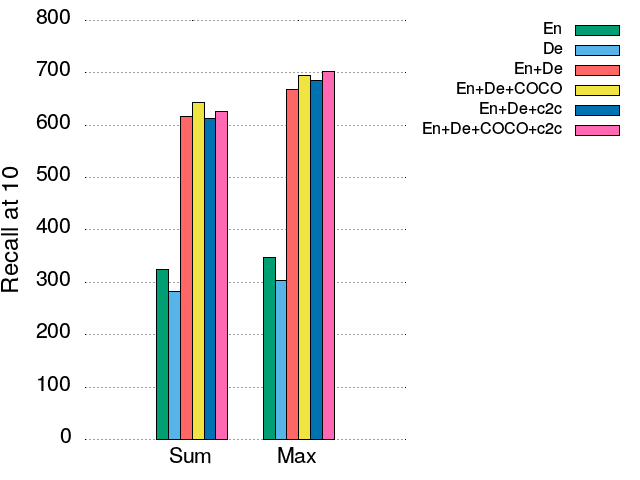
\includegraphics[scale=0.45]{assets/summax.png}
    \caption{Comparing Sum- and Max-violation loss. The reported values are the sum of recall scores 
            across R@1, R@5 and R@10 for both image-to-text and text-to-image retrieval for both English and german.
            Each value is the average of 3 runs.}
    \label{fig:summax}
\end{figure}